\chapter{SYSTEM ARCHITECTURE AND METHODOLOGY}

\section{System Block Diagram/Architecture}

\begin{figure}[H]
    \centering
    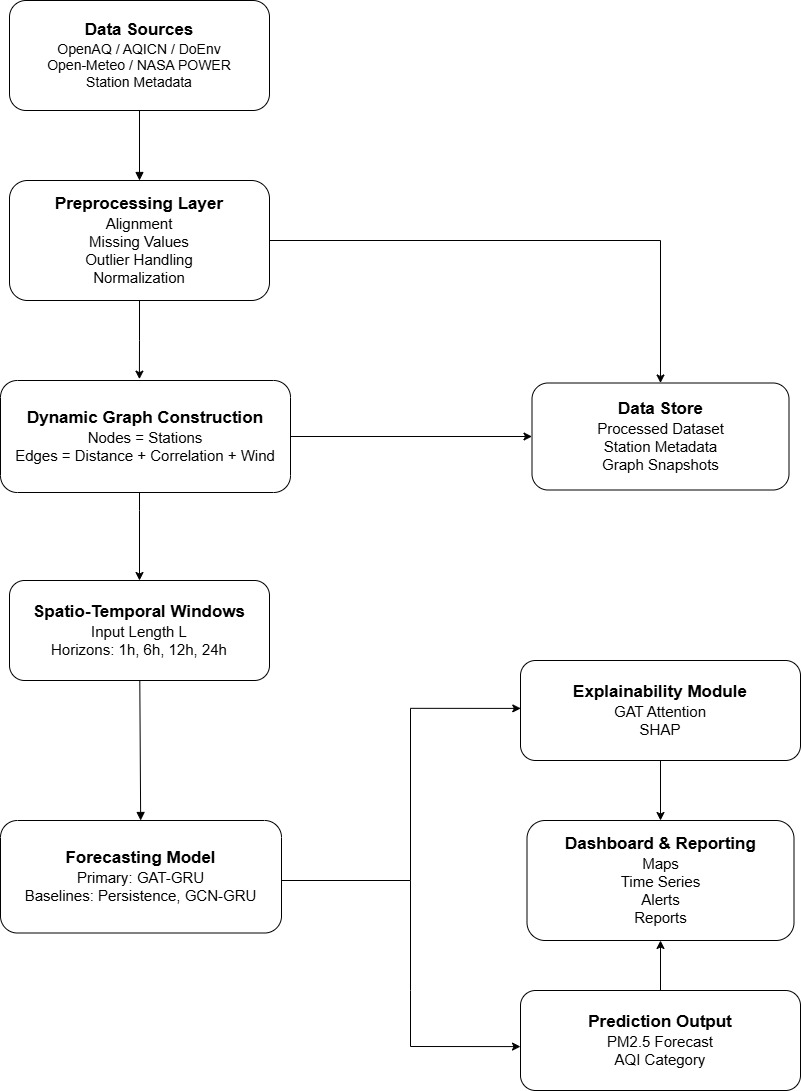
\includegraphics[width=\textwidth]{src/images/figures/sys_diagram.jpg}
    \caption{System Block Diagram}
    \label{fig:sys_diagram}
\end{figure}



\section{Description of Working Principle}

The proposed system works as a wind-aware air quality forecasting and decision-support system for short-term PM$_{2.5}$ prediction. It combines air quality data, meteorological data, dynamic graph construction, spatio-temporal deep learning, explainability, and dashboard-based visualization. The overall working principle of the system is described in the following subsections.

\subsection{Study Area, Stations and Data Access Status}

The initial study area for this project will be Kathmandu Valley, Nepal, covering major urban and semi-urban areas of Kathmandu, Lalitpur, and Bhaktapur. Kathmandu Valley is selected as the primary study area because it experiences high air pollution due to traffic emissions, construction activities, industrial sources, dust, seasonal variation, and its bowl-shaped geography, which can trap pollutants.

In the first stage of the project, the study will focus on selected air quality monitoring stations within Kathmandu Valley. These stations will be used to collect historical PM$_{2.5}$ observations, along with meteorological data such as wind speed, wind direction, temperature, humidity, and pressure where available.The initial proposal considered a small group of established Kathmandu Valley monitoring stations. Following automated station discovery through OpenAQ, the implementation identified 49 stations with at least some usable PM2.5 observations. However, these stations have substantially different monitoring periods and levels of temporal coverage. Therefore, the graph-modeling stage will select a core subset of stations with sufficient overlapping observations, while lower-coverage stations will be analyzed separately or included through masking where feasible.

For model development, each monitoring station will be represented as a node in a graph. The relationship between stations will be defined using factors such as geographical distance, wind direction, wind speed, and pollutant similarity.

\subsection{Dataset Description}

The currently prepared station datasets use PM$_{2.5}$ concentration as the target variable and meteorological variables as input features. Wind speed, wind direction, atmospheric pressure, humidity, temperature, precipitation, and dew point obtained from the Open-Meteo API will be considered as meteorological features. Wind speed and wind direction are particularly important for modeling the transport of airborne pollutants between monitoring stations. The spatial graph will therefore account for both geographical proximity and time-varying meteorological conditions.

\Cref{tab:integrated_dataset_sample} presents the proposed structure of the integrated dataset. The values are illustrative examples included only to demonstrate the organization of the model-ready records.

\begin{table}[H]
    \centering
    \small
    \caption{Illustrative Sample of the Integrated Dataset}
    \label{tab:integrated_dataset_sample}
    \renewcommand{\arraystretch}{1.2}
    \setlength{\tabcolsep}{4pt}

    \begin{tabularx}{0.94\linewidth}{|
        >{\raggedright\arraybackslash}p{2.6cm}|
        >{\raggedright\arraybackslash}p{2.0cm}|
        >{\centering\arraybackslash}p{1.5cm}|
        >{\centering\arraybackslash}p{1.5cm}|
        >{\centering\arraybackslash}p{1.5cm}|
        >{\raggedright\arraybackslash}X|}
        \hline
        \textbf{Timestamp} & \textbf{Station} & \textbf{PM$_{2.5}$} & \textbf{Temp.} & \textbf{Wind Spd.} & \textbf{Other Features} \\
        \hline

        2026-01-01 01:00 &
        Ratnapark &
        72.4 &
        5.3 &
        1.8 &
        RH, temperature, pressure, dew point, wind direction \\
        \hline

        2026-01-01 01:00 &
        Khumaltar &
        58.7 &
        5.1 &
        2.1 &
        RH, temperature, pressure, dew point, wind direction \\
        \hline

        2026-01-01 01:00 &
        Bhaktapur &
        64.9 &
        4.7 &
        1.5 &
        RH, temperature, pressure, dew point, wind direction \\
        \hline

    \end{tabularx}
\end{table}

In \Cref{tab:integrated_dataset_sample}, PM$_{2.5}$ concentration is expressed in $\mu g/m^3$, relative humidity is expressed as a percentage, temperature and dew point are expressed in degrees Celsius, atmospheric pressure is expressed in hPa, wind speed is expressed in m/s, and wind direction is expressed in degrees. The displayed values are illustrative rather than actual observations.

\subsection{Input Variables, Resolution and Prediction Target}

The proposed model will use hourly air quality and meteorological observations from multiple monitoring stations. Let $N$ represent the number of monitoring stations and $F$ represent the number of input features. At each time step $t$, the observations are represented as a node feature matrix:

\begin{equation}
X_t \in \mathbb{R}^{N \times F}
\end{equation}

where each row represents a monitoring station and each column represents a pollutant, meteorological, or temporal feature.

To capture temporal patterns, the model will use a sliding window of past observations. The default input window will be 24 hours, with a 48-hour window also tested for comparison. The primary forecasting horizon is 6 hours. Additional horizons of 1, 12, and 24 hours will be tested for comparison.

The main input variables will include historical PM$_{2.5}$, temperature, humidity, wind speed, wind direction, precipitation, pressure, dew point, and temporal features such as hour of day, day of week, month, and season. Wind direction will be converted into sine and cosine components because it is a circular variable. Missingness indicators may also be added to show whether a value was observed or imputed.

The primary prediction target is future PM$_{2.5}$ concentration at each monitoring station. For station $i$ and forecasting horizon $h$, the target value is represented as:

\begin{equation}
y_i^{(t+h)}
\end{equation}

and the model prediction is represented as:

\begin{equation}
\hat{y}_i^{(t+h)}
\end{equation}

Therefore, the task is formulated as a regression problem, where the model learns to minimize the difference between actual and predicted PM$_{2.5}$ values across all stations and time steps. Although the model predicts numerical PM$_{2.5}$ values, air quality categories such as good, moderate, unhealthy, and hazardous will be generated later in the post-processing stage using standard AQI threshold values.

\subsection{Data Preprocessing}

The collected air quality and meteorological data undergo a preprocessing stage before being used for graph construction and model training. Since the data are obtained from multiple sources, including OpenAQ and Open-Meteo, preprocessing is necessary to ensure consistency, reliability, and compatibility across all monitoring stations and environmental variables.

Air quality observations and meteorological records are first aligned according to their timestamps. Since the proposed system operates on hourly observations, all records are resampled and synchronized to a common hourly interval. For each monitoring station, PM$_{2.5}$, temperature, humidity, wind speed, wind direction, pressure, precipitation, and dew point measurements corresponding to the same timestamp are merged into a unified observation record. This temporal alignment ensures that all input variables represent the same environmental conditions at a given time step and prevents inconsistencies during model training.

The collected datasets are inspected for missing observations. Any missing values identified within the pollutant or meteorological variables are handled using appropriate interpolation techniques. Short gaps in continuous measurements are filled through linear interpolation, while larger missing segments may be removed if sufficient neighboring information is unavailable. This process helps preserve temporal continuity while reducing information loss caused by incomplete observations.

Environmental monitoring data may contain abnormal values caused by sensor malfunctions, communication errors, or measurement noise. Therefore, the dataset is examined for unrealistic or extreme observations. Basic statistical analysis and visualization techniques are used to identify potential outliers. Records containing physically impossible values, such as negative pollutant concentrations or invalid meteorological measurements, are removed or corrected according to data quality guidelines using either capping or log transformation.

The collected variables have different numerical ranges and units. To ensure stable neural network training, all numerical features are normalized before being supplied to the forecasting model. Min-Max normalization is applied to transform each feature into a common numerical range between 0 and 1. The normalized value of each feature is computed as:

\begin{equation}
X_{norm} = \frac{X - X_{min}}{X_{max} - X_{min}}
\end{equation}

where $X$ represents the original feature value, $X_{min}$ is the minimum observed value, and $X_{max}$ is the maximum observed value within the training dataset.

After preprocessing and normalization, the sequential observations are converted into fixed-length temporal windows for forecasting. A sliding-window approach is used to construct input sequences from historical observations. For example, if a 24-hour look-back period is selected, the model receives historical PM$_{2.5}$ and meteorological observations from the previous 24 hours and predicts the PM$_{2.5}$ concentration for the next forecasting horizon.

The final output of the preprocessing stage is a clean, synchronized, normalized, and temporally structured dataset containing station-wise pollutant and meteorological observations. These processed records are subsequently used for dynamic graph construction and spatio-temporal forecasting.

\subsection{Wind-Aware Dynamic Graph Construction}

The proposed system models air quality monitoring stations as a dynamic graph in order to capture spatial and meteorological dependencies among different locations within Kathmandu Valley. Unlike conventional static graphs that use only fixed geographical distance or historical correlation, the proposed approach constructs a wind-aware dynamic graph that adapts edge relationships based on time-varying meteorological conditions.

Let the air quality monitoring network be defined as a graph:

\begin{equation}
G_t = (V, E_t, A_t)
\end{equation}

where $V$ represents the set of monitoring stations, $E_t$ represents the set of edges at time $t$, and $A_t$ represents the adjacency matrix at time $t$. Each node $v_i \in V$ corresponds to a monitoring station and is associated with a feature vector:

\begin{equation}
X_i^t = [PM_{2.5}, Temperature, Humidity, WindSpeed, WindDirection, Pressure, DewPoint]
\end{equation}

An edge between two stations $i$ and $j$ is defined based on geographical distance, historical pollutant correlation, wind speed, and wind direction alignment. Thus, the edge weight is defined as a composite function:

\begin{equation}
A_{ij}^t = f_d(i,j) \cdot f_c(i,j) \cdot f_w(i,j,t)
\end{equation}

Spatial proximity between stations is modeled using normalized inverse distance:

\begin{equation}
f_d(i,j) = \exp\left(-\frac{d_{ij}}{\sigma_d}\right)
\end{equation}

where $d_{ij}$ is the geographical distance between stations $i$ and $j$, and $\sigma_d$ is a scaling parameter controlling spatial decay.

To capture long-term similarity in pollution patterns, historical correlation is computed as:

\begin{equation}
f_c(i,j) = \operatorname{corr}(PM_{2.5,i}, PM_{2.5,j})
\end{equation}

The key contribution of the proposed system is the incorporation of wind-driven pollutant transport. Wind influence is modeled as:

\begin{equation}
f_w(i,j,t) = \alpha \cdot \cos(\theta_{ij} - \theta_t) \cdot WS_t
\end{equation}

where $\theta_{ij}$ is the direction from station $i$ to station $j$, $\theta_t$ is the wind direction at time $t$, $WS_t$ is the wind speed at time $t$, and $\alpha$ is a scaling factor. This formulation increases influence when wind flows from one station toward another, decreases influence when wind flows in the opposite direction, and amplifies spatial propagation effects during stronger wind conditions.

The final adjacency matrix is time-dependent and is updated at every time step to reflect changing meteorological conditions:

\begin{equation}
A_t =
\begin{bmatrix}
A_{11}^t & A_{12}^t & \cdots & A_{1n}^t \\
A_{21}^t & A_{22}^t & \cdots & A_{2n}^t \\
\vdots & \vdots & \ddots & \vdots \\
A_{n1}^t & A_{n2}^t & \cdots & A_{nn}^t
\end{bmatrix}
\end{equation}

The output of this module is the dynamic adjacency matrix $A_t$, the node feature matrix $X_t$, and the edge-weighted graph representation $G_t$. These outputs are subsequently used as input to the graph attention layer for spatial feature learning.

\subsection{Virtual Node Construction for Unmonitored Locations}

A key novelty of this project is the use of virtual nodes to estimate air pollution at locations where physical air quality monitoring stations are not available. In real-world settings, monitoring stations are limited and cannot represent every road, neighborhood, or residential area. To address this limitation, the proposed system will allow selected map locations to be represented as virtual nodes within the graph.

A virtual node represents an unmonitored geographic location selected from the map. Unlike physical stations, this node does not have direct sensor readings. Therefore, its initial feature values will be estimated using information from nearby monitoring stations. For a completely new virtual location, edge construction will use only information genuinely available at deployment time, including coordinates, distance, meteorological conditions, and optional static geographical attributes. Historical PM2.5 correlation will not be used because the virtual location has no pollutant observations. During training, randomly masked real stations will be treated as virtual nodes so that the model learns to infer node representations without using their PM2.5 history. Stations that are closer or located along the wind flow direction will be assigned stronger influence.

Formally, if there are $N$ real monitoring stations and $V$ virtual nodes, the graph is expanded as:

\begin{equation}
N' = N + V
\end{equation}

where $N'$ is the total number of real and virtual nodes in the graph. The model then performs prediction over both physical monitoring stations and virtual nodes.

The virtual node mechanism enables the system to estimate PM$_{2.5}$ concentration at unmonitored locations and generate a more continuous air pollution map. This is useful for identifying pollution patterns in areas without sensors and for improving the practical usability of the forecasting system.

To validate this approach, a leave-one-station-out strategy may be used. In this method, one real station is temporarily treated as a virtual node, and its actual PM$_{2.5}$ values are hidden from the model during prediction. The predicted values are then compared with the actual station readings. This allows the performance of virtual-node-based prediction to be evaluated even when real ground truth is not available for completely unmonitored locations.

\subsection{Spatio-Temporal Forecasting Model}

The proposed system employs a hybrid Graph Attention Network and Gated Recurrent Unit architecture to model both spatial and temporal dependencies in air quality data. This combination enables the model to capture pollutant interactions across monitoring stations as well as temporal variations over time.

In addition to forecasting PM$_{2.5}$ at physical monitoring stations, the model will also support prediction at virtual nodes. These virtual nodes represent unmonitored map locations and are connected to the existing station graph using wind-aware spatial relationships. This allows the GAT-GRU model to estimate pollution levels beyond the available sensor network.

At each time step $t$, the model receives a node feature matrix:

\begin{equation}
X_t \in \mathbb{R}^{N \times F}
\end{equation}

and a dynamic adjacency matrix:

\begin{equation}
A_t \in \mathbb{R}^{N \times N}
\end{equation}

where $N$ represents the number of monitoring stations and $F$ represents the number of input features per station. The adjacency matrix is generated from the wind-aware graph using factors such as geographical distance, wind direction, wind speed, and pollutant similarity.

The Graph Attention Network captures spatial influence between monitoring stations. For each station $i$, the GAT layer aggregates information from neighboring stations using attention weights:

\begin{equation}
h_i^t = \sigma \left( \sum_{j \in \mathcal{N}(i)} \alpha_{ij}^t W x_j^t \right)
\end{equation}

where $x_j^t$ is the feature vector of neighboring station $j$, $W$ is a learnable weight matrix, $\alpha_{ij}^t$ is the attention coefficient, $\mathcal{N}(i)$ represents the neighboring stations of station $i$, and $\sigma$ is a non-linear activation function. The attention coefficient $\alpha_{ij}^t$ shows how much influence station $j$ has on station $i$ at time $t$. This also supports model explainability because the learned attention weights can help identify which nearby stations contribute most to a prediction.

The wind-aware adjacency matrix determines the valid directed edges and provides an edge attribute representing physical transport plausibility. The GAT subsequently learns data-driven attention over these permitted edges. Thus, the wind-aware weight acts as a physical prior, while the attention coefficient represents the model’s learned importance. In implementation, the wind-aware edge weight will either be concatenated with the attention input or used to modulate the pre-softmax attention score. These two configurations will be compared experimentally.

\begin{figure}[H]
    \centering
    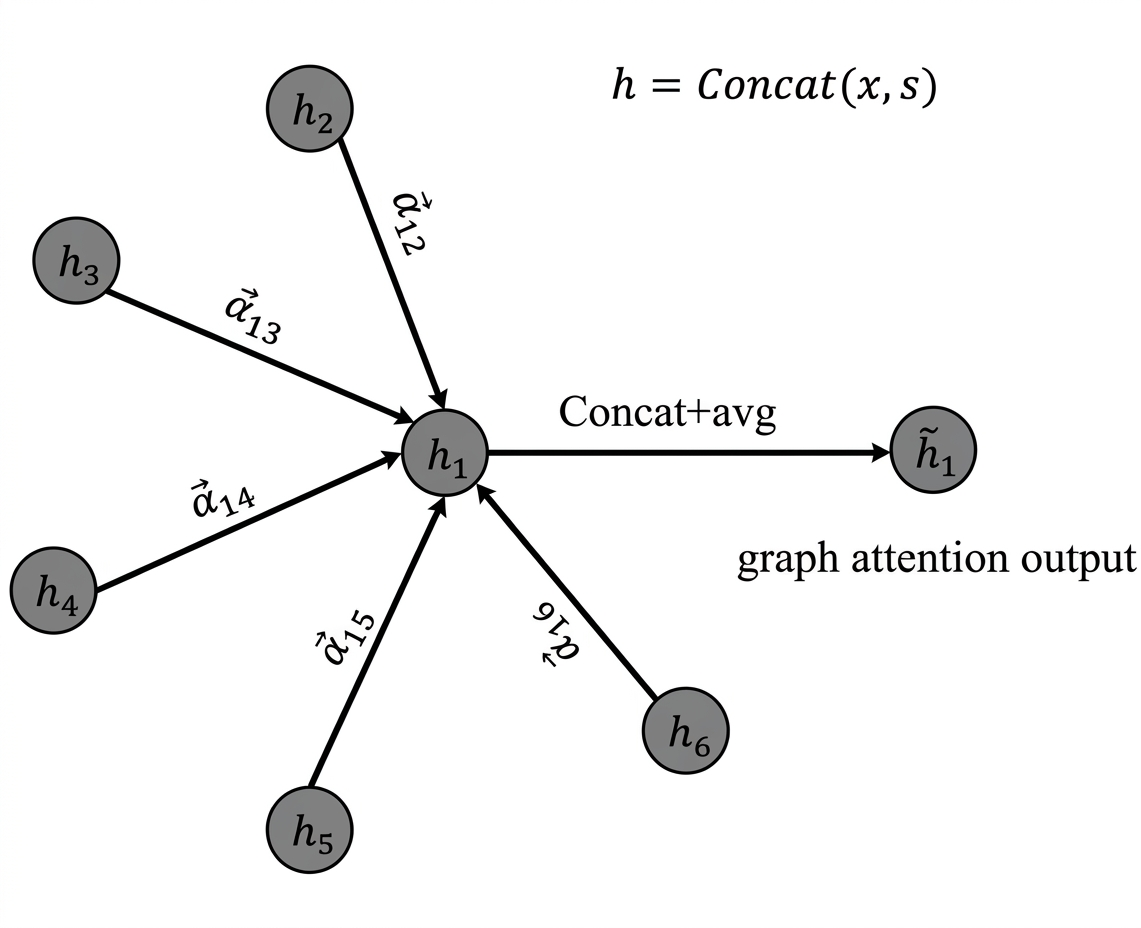
\includegraphics[width=0.92\textwidth]{src/images/figures/spatial_modeling.png}
    \caption{Spatial modeling using graph attention}
    \label{fig:spatial_modeling}
\end{figure}

The spatial output of the GAT layer is represented as:

\begin{equation}
H_t = GAT(X_t, A_t)
\end{equation}

To capture temporal dependencies, the spatial embeddings from multiple previous time steps are passed into a GRU network. For an input window of length $L$, the GRU processes:

\begin{equation}
H_{t-L+1:t}
\end{equation}

The hidden state is updated as:

\begin{equation}
z_t = GRU(H_t, z_{t-1})
\end{equation}

where $H_t$ is the spatial embedding at time $t$, and $z_t$ is the hidden state that captures temporal evolution. This allows the model to learn short-term pollution changes, delayed meteorological effects, and temporal persistence in PM$_{2.5}$ concentration.

\begin{figure}[H]
    \centering
    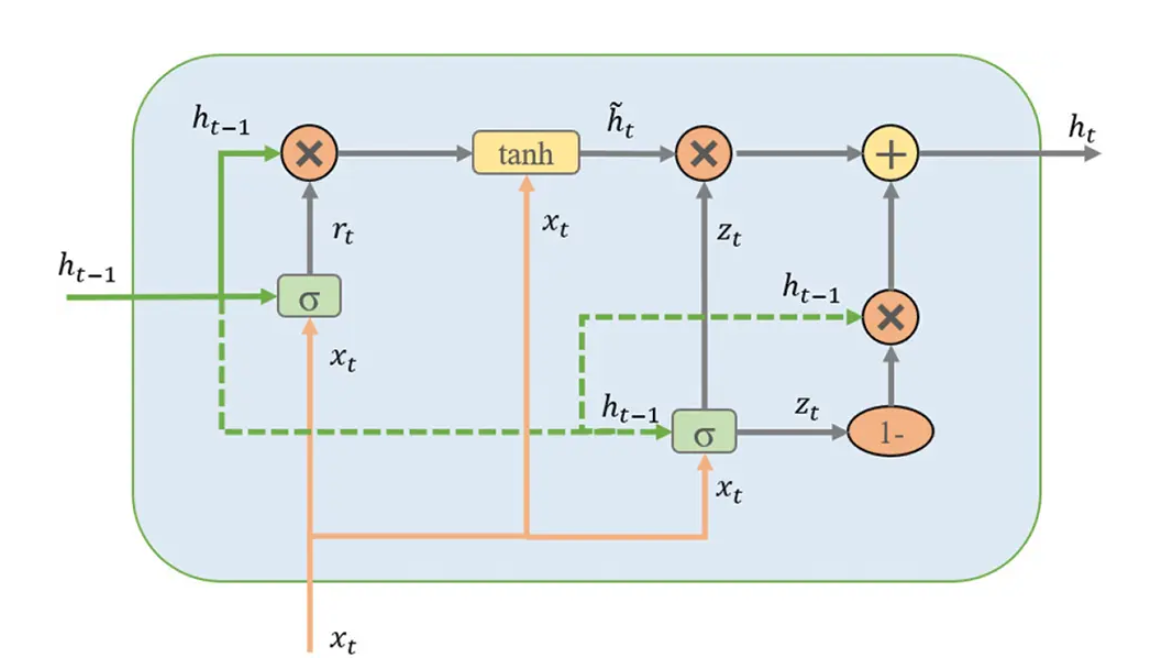
\includegraphics[width=0.92\textwidth]{src/images/figures/temporal_modeling.png}
    \caption{Temporal modeling using GRU}
    \label{fig:temporal_modeling}
\end{figure}

The final hidden representation from the GRU is passed through a fully connected regression layer to predict future PM$_{2.5}$ concentration at each station:

\begin{equation}
\hat{y}_{t+h} = W_o z_t + b
\end{equation}

where $\hat{y}_{t+h}$ is the predicted PM$_{2.5}$ concentration after horizon $h$, and $h \in \{1, 6, 12, 24\}$. The one-hour horizon represents the single-step forecasting case, while 6, 12, and 24-hour horizons are used for multi-horizon forecasting. The overall architecture can be summarized as input features, wind-aware graph construction, GAT layer, GRU layer, and regression output.

\subsection{Explainability Module}

The proposed system includes an explainability module to help interpret the predictions generated by the wind-aware spatio-temporal forecasting model. Since the model uses GAT and GRU layers, the explanation focuses on spatial influence, feature contribution, and temporal importance.

Spatial explainability is obtained from the attention weights learned by the GAT layer. For a target station or virtual node, the attention coefficient $\alpha_{ij}$ shows how much neighboring station $j$ contributes to the prediction at node $i$. These attention values help identify the most influential stations, possible pollutant movement direction, and the effect of wind-aware graph connections. This is especially useful when estimating PM$_{2.5}$ at virtual nodes, as it can show which real monitoring stations influenced the predicted value.

Feature-level explainability will be analyzed using SHAP or similar feature importance methods. This will help identify how much each input variable, such as historical PM$_{2.5}$, wind speed, wind direction, temperature, humidity, pressure, dew point, and temporal features, contributes to the final prediction. This allows the system to explain why a predicted pollution value is high or low.

Temporal interpretability will be studied by analyzing how different historical time windows affect the forecast. Since the GRU learns from past observations, this analysis helps understand whether the prediction is mainly influenced by recent pollution spikes, delayed weather effects, or persistent pollution patterns.

The explainability outputs will be presented through visualizations such as station influence maps, attention-based graph plots, feature importance charts, and time-series plots. These explanations will make the model more transparent and useful for air quality monitoring, pollution interpretation, and decision support.

\clearpage
\begin{samepage}
\section{Flow Diagram}

\begin{figure}[H]
    \centering
    \begin{tikzpicture}[
        node distance=8mm,
        startstop/.style={
            ellipse,
            draw,
            align=center,
            minimum width=4cm,
            minimum height=8mm
        },
        process/.style={
            rectangle,
            draw,
            align=center,
            minimum width=8.2cm,
            minimum height=8mm
        },
        arrow/.style={->, thick}
    ]

        % Nodes
        \node[startstop] (start) {Start};

        \node[process, below=of start] (collect) {Collect air quality and meteorological data};
        \node[process, below=of collect] (clean) {Clean missing and inconsistent values};
        \node[process, below=of clean] (align) {Align station data by timestamp};
        \node[process, below=of align] (graph) {Construct wind-aware dynamic graph};
        \node[process, below=of graph] (window) {Create input time windows};
        \node[process, below=of window] (train) {Train baseline and GAT-GRU models};
        \node[process, below=of train] (predict) {Predict future pollutant levels};
        \node[process, below=of predict] (evaluate) {Evaluate regression};
        \node[process, below=of evaluate] (explain) {Generate prediction explanations};
        \node[process, below=of explain] (display) {Display results on dashboard};

        \node[startstop, below=of display] (end) {End};

        % Arrows
        \draw[arrow] (start) -- (collect);
        \draw[arrow] (collect) -- (clean);
        \draw[arrow] (clean) -- (align);
        \draw[arrow] (align) -- (graph);
        \draw[arrow] (graph) -- (window);
        \draw[arrow] (window) -- (train);
        \draw[arrow] (train) -- (predict);
        \draw[arrow] (predict) -- (evaluate);
        \draw[arrow] (evaluate) -- (explain);
        \draw[arrow] (explain) -- (display);
        \draw[arrow] (display) -- (end);

    \end{tikzpicture}

    \caption{Proposed air quality forecasting workflow}
    \label{fig:air_quality_flowchart}
\end{figure}
\end{samepage}

\section{Instrumentation Tools}
\begin{table}[H]
    \centering
    \small
    \caption{Proposed Technical Stack}
    \label{tab:technical_stack}
    \renewcommand{\arraystretch}{1.2}
    \setlength{\tabcolsep}{4pt}

    \begin{tabularx}{0.94\linewidth}{|
        >{\raggedright\arraybackslash}p{3.0cm}|
        >{\raggedright\arraybackslash}X|}
        \hline
        \textbf{Category} & \textbf{Tools and Technologies} \\
        \hline

        Data Processing &
        Python, pandas, NumPy, scikit-learn \\
        \hline

        Deep Learning &
        PyTorch, PyTorch Geometric, SHAP \\
        \hline

        Forecasting Models &
        Persistence model, linear/tree regression, GRU, GAT-GRU \\
        \hline

        Data Sources &
        OpenAQ, Open-Meteo \\
        \hline

        Backend &
        FastAPI, Representational State Transfer (REST) services \\
        \hline

        Frontend &
        React, Leaflet or Mapbox, Recharts \\
        \hline

        Database and Storage &
        PostgreSQL, CSV/Parquet files, local storage for datasets, models, and experiment logs \\
        \hline

        Deployment &
        Docker, local server, optional cloud deployment \\
        \hline
    \end{tabularx}
\end{table}

\section{Evaluation Methodology}

\subsection{Evaluation Metrics}

The project will evaluate forecasting models using regression metrics and horizon-wise error analysis. The proposed GAT-GRU model will be compared with baseline models to check whether dynamic graph learning improves forecasting accuracy.

Mean Absolute Error (MAE) measures the average absolute prediction error in PM$_{2.5}$ values:

\begin{equation}
MAE = \frac{1}{n} \sum_{i=1}^{n} |y_i - \hat{y}_i|
\end{equation}

Root Mean Squared Error (RMSE) penalizes large errors more strongly and is useful for evaluating pollution spikes:

\begin{equation}
RMSE = \sqrt{\frac{1}{n} \sum_{i=1}^{n} (y_i - \hat{y}_i)^2}
\end{equation}

Mean Absolute Percentage Error (MAPE) measures prediction error in percentage form:

\begin{equation}
MAPE = \frac{1}{n} \sum_{i=1}^{n} \left|\frac{y_i - \hat{y}_i}{y_i}\right| \times 100
\end{equation}

The $R^2$ score shows how well the model explains variation in PM$_{2.5}$ concentration:

\begin{equation}
R^2 = 1 - \frac{\sum (y_i - \hat{y}_i)^2}{\sum (y_i - \bar{y})^2}
\end{equation}

Bias indicates whether the model generally overpredicts or underpredicts:

\begin{equation}
Bias = \frac{1}{n} \sum_{i=1}^{n} (y_i - \hat{y}_i)
\end{equation}


Explainability will be assessed qualitatively by inspecting whether important stations, weather factors, and time windows are consistent with wind direction, distance, and pollutant history. The dashboard will be evaluated based on whether it can clearly present forecasts, AQI categories, spatial maps, explanation visualizations, and what-if scenario comparisons.
